\section{Experiments}
\label{sec:experiments}

\subsection{Setup}
\label{sec:exp-setup}
\paragraph{Benchmark.}
We use AdaptiveQuadBench \citep{zhang2025adaptivequadbench} with RotorPy \citep{folk2023rotorpy} at 100\,Hz, on 5\,s random trajectories and its seven disturbance families: none, wind, external force, external torque, payload, rotor-effectiveness loss and parameter uncertainty.
For each family we run 20 trials with the benchmark's evaluation seed. Each regime therefore has 140 \emph{paired} trials, in which every controller sees the same vehicle, trajectory, disturbance and noise realisation.
On top of the benchmark we add seven sensing/fault regimes (details in App.~\ref{app:impl}): \emph{noise} (mocap/IMU-level Gaussian noise on all states and rotor speeds); \emph{heavy} (Student-$t$, $\nu{=}2.5$); \emph{outliers} (noise plus 2\%/step 20$\sigma$ glitches); \emph{dropout} (noise plus frozen packets of 50--200\,ms); \emph{impacts} (three kicks of 0.5--1.5\,m/s and 2--5\,rad/s); \emph{rotor flicker} (one rotor toggles between healthy and 30--60\% effectiveness every 0.2--0.8\,s); and \emph{stress} (all of the above with aggressive trajectories).

\paragraph{Baselines.}
\emph{Stock:} the seven controllers shipped with the benchmark, \emph{unmodified}: geometric \citep{lee2010geometric}, geometric-adaptive, $\mathcal{L}_1$-geometric \citep{wu2023l1quad}, adaptive INDI \citep{smeur2016adaptive,tal2021accurate}, MPC, $\mathcal{L}_1$-MPC and the learned XAdap \citep{zhang2024xadap}.
\emph{Strengthened:} because the stock controllers turn out to be far from \ours{}, we also built two strong baselines. They share \emph{everything} with \ours{} (NMPC, rotor-drag model, front end, offset-free input target) except the estimator: a tuned outlier-robust lumped KF \citep{ting2007kalman}, and multiple-model adaptive estimation (MMAE) \citep{magill1965optimal} over the same four-KF bank with forgetting. They isolate the value of the learned estimator.

\paragraph{Metrics and statistics.}
We report median position RMSE, counting a trial with RMSE $>1$\,m or divergence as a failure that is ranked worst. Comparisons use one-sided Wilcoxon signed-rank tests on the paired trials \citep{wilcoxon1945individual} and exact McNemar tests on paired unsafe outcomes \citep{mcnemar1947note}.
Learned estimators are averaged per trial over three training seeds.

\subsection{Tracking under disturbances and sensing faults}
\label{sec:exp-tracking}


\begin{table}[t]
  \centering\small
  \caption{Median position RMSE [cm] per regime (140 paired trials each). Superscripts give the success rate when below 100\%. Bold marks the best NMPC variant. The gain and wins compare \ours{} (GDN, three-seed mean) with the \emph{best} stock controller in that regime, chosen post hoc; all $p<10^{-6}$ (one-sided Wilcoxon).}
  \label{tab:main}
  \resizebox{\linewidth}{!}{\begin{tabular}{l l r r r r r r r}
\toprule
 & \multicolumn{2}{c}{Best stock controller} & NMPC+ & NMPC+ & \multicolumn{2}{c}{\textbf{ICON-MPC (ours)}} & \multicolumn{2}{c}{GDN vs.\ best stock} \\
\cmidrule(lr){2-3}\cmidrule(lr){6-7}\cmidrule(lr){8-9}
Regime & name & RMSE & rob.\ KF & MMAE & Mamba & GDN & gain & wins \\
\midrule
Base & INDI-A & 3.18 & 0.52 & \textbf{0.40} & 0.41 & 0.46 & 7.0$\times$ & 140/140 \\
Gauss.\ noise & L1-MPC & 3.92 & 1.00 & 1.65 & \textbf{0.91} & 0.97 & 4.1$\times$ & 140/140 \\
Heavy-tail & L1-MPC & 4.50 & 0.98 & 1.26 & \textbf{0.84} & 0.91 & 4.9$\times$ & 140/140 \\
Outliers & XAdap & 6.32 & 1.19 & 1.68 & \textbf{1.15} & 1.18 & 5.3$\times$ & 140/140 \\
Dropout & Geo-adaptive & 12.12$^{\,99\%}$ & 2.31 & 3.60 & \textbf{1.77} & 1.83 & 6.6$\times$ & 140/140 \\
Rotor flicker & INDI-A & 3.64 & 1.11 & 1.11 & \textbf{0.63} & 0.74 & 5.0$\times$ & 140/140 \\
Impacts & MPC & 9.95 & \textbf{5.92$^{\,95\%}$} & 6.00 & 6.52 & 7.04 & 1.4$\times$ & 124/140 \\
Stress (all) & XAdap & 59.30$^{\,73\%}$ & 11.06$^{\,92\%}$ & 11.25$^{\,96\%}$ & 10.36 & \textbf{10.00$^{\,99\%}$} & 5.9$\times$ & 138/140 \\
\bottomrule
\end{tabular}
}
\end{table}

\paragraph{Against the benchmark's controllers.}
Table~\ref{tab:main} (and Fig.~\ref{fig:tracking}, App.~\ref{app:results}) shows that \ours{} reduces the median RMSE by $4.1$--$7.0\times$ relative to the best stock controller in every regime except impacts. It wins 138--140 of 140 paired trials ($p<10^{-6}$).
Under combined stress, the best stock controller (XAdap) succeeds in 73\% of trials and \ours{} in 99\%.
Impacts are the exception ($1.4\times$, 124/140 wins). An impact is a state jump rather than a persistent disturbance, so little remains to be estimated, and all NMPC variants are within 20\% of each other.
Outside impacts, even the strengthened KF baseline is $3.3$--$6.1\times$ better than the best stock controller, which motivates the strengthened comparison.


\paragraph{Against strengthened baselines.}
Here only the estimator differs (Table~\ref{tab:main}; per-regime tests in Table~\ref{tab:strong}, App.~\ref{app:results}). The learned estimator is significantly better where the KF assumptions break hardest: packet dropout ($1.26\times$, 117/140 wins), rotor flicker ($1.50\times$; a switching, input-dependent disturbance, the setting of Proposition~\ref{prop:nlms}) and combined stress ($1.11\times$, with success rising from 92.1\% (KF) and 96.4\% (MMAE) to 98.6\%).
The gains are smaller but significant under Gaussian noise, heavy-tailed noise and outliers ($1.01$--$1.07\times$, $p\le 0.013$).
\ours{} does \emph{not} win in two regimes. In the nominal base regime, MMAE is better ($0.87\times$): with clean sensing a bank of well-tuned KFs is near-optimal (Fact~1 in App.~\ref{app:proofs}). Under impacts, the robust KF is better ($0.84\times$) because it reacts to state jumps more conservatively.
Mamba matches or slightly beats GDN in most regimes (per-seed results in App.~\ref{app:results}). We thus do \emph{not} claim GDN is the better drop-in sequence model; its distinguishing feature is the structure of Proposition~\ref{prop:nlms}.

\paragraph{Compute.}
\ours{} takes 3.9\,ms per step on average (6.5\,ms at the 99th percentile) on one CPU thread, within the 10\,ms budget. Stock controllers are $10\times$ cheaper but far less accurate (Table~\ref{tab:compute}, App.~\ref{app:results}).

\subsection{Safety under state constraints: obstacles that intrude into the path}
\label{sec:exp-obstacles}

\paragraph{Scenario.}
We place four vertical cylinders (radius 0.1--0.3\,m plus a 0.1\,m body radius) at least 15\,cm apart, such that the reference \emph{cuts 3--10\,cm into each inflated obstacle}. Tracking the reference blindly therefore guarantees a collision, and the controller must trade tracking for clearance.
We test four regimes: base, noise, rotor flicker and stress (noise, outliers, dropout and flicker together), each with 140 paired trials. The stock controllers have no constraint interface and are shown for reference only.
The constrained baselines use the same soft constraints \eqref{eq:ocp} with either no margin, a fixed 3\,cm margin, or the ACI margin \eqref{eq:aci}.

\begin{figure}[t]
  \centering
  \begin{minipage}[c]{0.66\linewidth}
    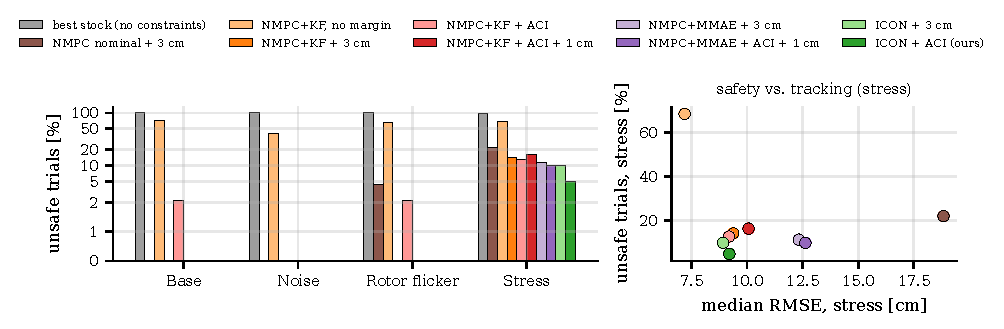
\includegraphics[width=\linewidth]{figures/obstacle_safety.pdf}
  \end{minipage}\hfill
  \begin{minipage}[c]{0.32\linewidth}
    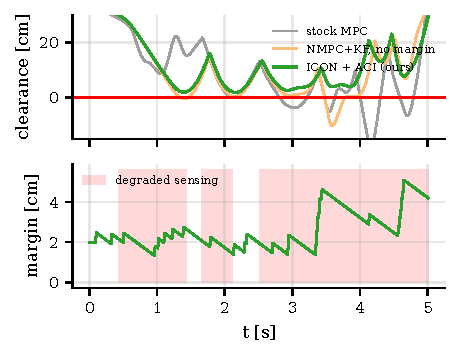
\includegraphics[width=\linewidth]{figures/aci_margin.pdf}
  \end{minipage}
  \caption{\emph{Left:} unsafe-trial rate (collision or failure; symlog scale) and the safety--tracking trade-off under stress. \emph{Right:} one stress trial (wind). Top: clearance to the nearest inflated obstacle; below the red line is a collision. Bottom: the ACI margin $\mu_t$ of \ours{}, which grows during degraded-sensing episodes (shaded) and decays afterwards.}
  \label{fig:obstacles}\label{fig:aci}
\end{figure}


\paragraph{Results.}
\emph{Constraints and margins are necessary:} the stock controllers collide in essentially every trial, and the constrained KF-NMPC without a margin is unsafe in 41--73\% of trials, because noise and estimation error push the realised trajectory over the boundary the plan merely touches.
\emph{Without combined faults, every calibrated margin suffices:} with base, noise or flicker sensing, every margin of 3\,cm or ACI\,+\,1\,cm is safe in all 140 trials, and among these \ours{} tracks best (6.2, 8.0 and 6.3\,cm) because its margin shrinks when tracking is accurate.
\emph{Under combined faults, \ours{} is the safest:} under stress, \ours{} is unsafe in 5.0\% of trials versus 10.0--22.1\% for every other constrained controller (Table~\ref{tab:obstacles}, App.~\ref{app:results}). This is significant against all KF-based and nominal variants, including KF\,+\,ACI with the same floor (16.4\%, $p=2\cdot10^{-4}$), and against MMAE with a 3\,cm margin ($p=0.04$). Against MMAE\,+\,ACI\,+\,1\,cm (10.0\%) the difference is not significant ($p=0.08$), but that baseline tracks 37\% worse (12.6 vs.\ 9.2\,cm). Time in collision falls to 0.07\%, from 0.27\% (MMAE\,+\,ACI) and 0.46\% (KF\,+\,ACI\,+\,1\,cm).
\emph{Calibration matches the theory:} the realised ACI miss frequency is 4.3--5.4\% in every regime and for every estimator, against the target $\alpha=5\%$, as predicted by Theorem~\ref{thm:aci}. The estimator matters because it makes the plan \emph{more predictable}, so the same coverage needs a smaller margin. Figure~\ref{fig:snapshots} (App.~\ref{app:results}) shows a 3D rollout.

\subsection{Ablations}
\label{sec:ablation}
Table~\ref{tab:ablation} (App.~\ref{app:results}) shows that an NMPC \emph{without} disturbance estimation (4--5\,cm, even with rotor drag) is no better than the best stock controller; offset-free estimation with the robust KF alone gives $2.2$--$7.7\times$. Sequence models add on top where KF assumptions fail, and only the selective ones (Mamba, GDN) also help with clean sensing. Removing the front end is catastrophic under dropout (81\% success) and stress (58\%).
